
\label{cap_resultados}

\indent

Apresentamos neste capítulo a metodologia empregada e os resultados experimentais obtidos ao testar se fórmulas menores produzem respostas mais rápido e ao comparar algoritmos para escolha de renomeamento.

\section{Metodologia}

\indent

Apresentamos nesta seção os detalhes necessários para reproduzir os experimentos realizados.

\subsection{Representações de fórmulas}

\indent

A forma que utilizamos para representar fórmulas lógicas em textos teóricos, ou seja, cadeias da respectiva linguagem formal, se mostra pouco prática para implementar transformações ou algoritmos de busca.

Observe, no entanto, que definimos a linguagem formal da lógica proposicional como uma \emph{gramática livre-do-contexto} \cite{sipser2012introduction} e, portanto, é garantido que temos um algoritmo de custo de tempo polinomial determinístico para obter a \emph{árvore sintática}, ou simplesmente \emph{árvore}, de uma fórmula \cite{younger1967recognition}. Tal estrutura se mostra muito mais prática para a implementação de algoritmos de transformação e busca do que cadeias de linguagens formais.

Ainda melhor que árvores para representar fórmulas, são \emph{grafos acíclicos dirigidos}, ou simplesmente DAGs na sigla do inglês, onde os vértices que representam subfórmulas distintas compartilham arestas com o vértice de uma mesma subfórmula que ambas possuem em comum \cite{jackson2004clause}. Tais estruturas equivalem a representar o conjunto de subfórmulas de fato como um conjunto, ou seja, $|\{\psi \in SF(\phi) \mid \psi = \xi \}| = 1$, para todas $\phi$ e $\xi \sqsubseteq \phi$. É então uma forma de representação oposta a árvores, que representam o conjunto de subfórmulas como um multiconjunto, ou seja, é possível acontecer $|\{\psi \in SF(\phi) \mid \psi = \xi \}| > 1$. Em outras palavras, árvores sempre representam fórmulas como se nunca houvesse repetição de subfórmulas, criando cópias distintas para as distintas posições em que uma mesma subfórmula ocorre, enquanto DAGs permitem uma representação ``honesta'', ou seja, repetições de subfórmulas podem ser consideradas e cada subfórmula é representada por um único objeto (vértice). Além disso, DAGs são exponencialmente menores que árvores no melhor caso, como mostra a Figura \ref{figura_DAG}, e, portanto, propícios a algoritmos de programação dinâmica \cite{bellman2015applied} exponencialmente mais rápidos no melhor caso.

\begin{figure}
	\centering
	
	\raisebox{3.5\height}{$(p \leftrightarrow p) \leftrightarrow (p \leftrightarrow p)$}
	\hspace{1cm}
	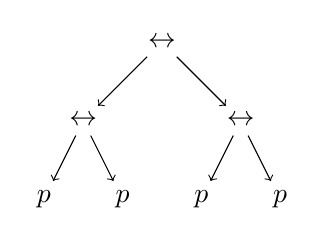
\begin{tikzpicture}
	\tikzset{vertex/.style = {}}
	\tikzset{edge/.style = {->}}
	
	\node[vertex]  (1) at (   0,    1) {$\leftrightarrow$};
	\node[vertex]  (2) at (  -1,    0) {$\leftrightarrow$};
	\node[vertex]  (3) at (   1,    0) {$\leftrightarrow$};
	\node[vertex]  (4) at (-1.5,   -1) {$p$};
	\node[vertex]  (5) at (-0.5,   -1) {$p$};
	\node[vertex]  (6) at ( 0.5,   -1) {$p$};
	\node[vertex]  (7) at ( 1.5,   -1) {$p$};
	
	\draw[edge] (1) to  (2);
	\draw[edge] (1) to  (3);
	\draw[edge] (2) to  (4);
	\draw[edge] (2) to  (5);
	\draw[edge] (3) to  (6);
	\draw[edge] (3) to  (7);
	\end{tikzpicture}
	\hspace{2cm}
	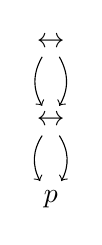
\begin{tikzpicture}
	\tikzset{vertex/.style = {}}
	\tikzset{edge/.style = {->}}
	
	\node[vertex]  (1) at (   0,    1) {$\leftrightarrow$};
	\node[vertex]  (2) at (   0,    0) {$\leftrightarrow$};
	\node[vertex]  (3) at (   0,   -1) {$p$};
	
	\draw[edge] (1) to [bend right] (2);
	\draw[edge] (1) to [bend left ] (2);
	\draw[edge] (2) to [bend right] (3);
	\draw[edge] (2) to [bend left ] (3);
	\end{tikzpicture}
	
	\hspace{1.45cm}(a)\hspace{4.2cm}(b)\hspace{3.85cm}(c)
	
	\label{figura_DAG}
	\caption{Representações de $(p \leftrightarrow p) \leftrightarrow (p \leftrightarrow p)$. (a) Cadeia. (b) Árvore. (c) DAG.}
\end{figure}

As três formas de representação de fórmulas apresentadas nesta seção são utilizadas em diferentes etapas da implementação, como discutimos a seguir.

\subsection{Implementação}

\indent

Implementamos um programa, utilizando a linguagem de programação C++ versão 11, que recebe uma fórmula sob a forma de cadeia, realiza uma série de transformações e dá como saída uma fórmula resultante também sob a forma de cadeia, juntamente com três medidas desta última fórmula: seu tamanho, número de cláusulas e número de símbolos proposicionais. As transformações realizadas são detalhadas a seguir. Optamos por deixar flexível a execução ou não de algumas transformações, mas fixamos a ordem em que as transformações são realizadas.

\subsubsection{Análise sintática}

\indent

Convertemos uma fórmula sob a forma de cadeia para uma árvore sintática. Implementamos um algoritmo de pilha que faz uma única varredura na cadeia e produz a árvore. Esta transformação é sempre executada.

\subsubsection{Conversão para FNN}

\indent

A próxima transformação coloca a fórmula na forma normal negada. Realizamos esta transformação por dois motivos em particular:
\begin{enumerate}
	\item As versões dos algoritmos para escolha de renomeamento e do algoritmo de conversão para a FNC são extremamente mais simples para fórmulas na FNN;
	\item Optando por não realizar a conversão para DAG mais adiante, a transformação que obtemos simula uma árvore linear. É claro que, em geral, as fórmulas não são necessariamente árvores lineares. No entanto, se for representada por uma árvore sintática, qualquer fórmula na FNN é considerada uma árvore linear pelos algoritmos de renomeamento. Portanto, podemos testar casos em que os algoritmos não necessariamente escolhem renomeamentos ótimos, mas necessariamente escolhem renomeamentos que geram o mesmo número de cláusulas.
\end{enumerate}

Esta transformação é necessária somente para a realização de renomeamento e conversão para FNC. Pode ser desligada, caso o objetivo da execução do programa seja apenas obter as medidas da fórmula original.

\subsubsection{Aplainamento}

\indent

Aplicamos aplainamento à exaustão. Isto não é necessário para nenhuma outra transformação e portanto pode-se optar por não realizar aplainamento. No entanto, esta transformação faz com que apareçam mais situações em que é possível aplicar simplificação \cite{sebastiani2009automated}. E, ainda, no contexto de renomeamento, o exemplo a seguir evidencia como aplainamento pode ser proveitoso.

Considere $\phi$ da forma $(p \wedge (q \wedge r)) \vee ... \vee ((p \wedge q) \wedge r)$. Na forma aplainada de $\phi$, $(p \wedge q \wedge r)$ pode ser renomeada por um único novo símbolo proposicional em suas duas ocorrências.

\subsubsection{Conversão para DAG}

\indent

A conversão é feita através de um algoritmo ascendente, ou seja, construímos o DAG de baixo para cima, indo em direção à raiz da árvore. Esta transformação não é necessária para nenhuma transformação seguinte e é possível optar por não executá-la.

Vale observar ainda que optamos por executar a conversão para DAG somente após colocar a fórmula na FNN, dado que isto evita o seguinte problema.

Suponha que $\psi$ ocorra em $\pi_1 \in pos(\phi)$ e em $\pi_2 \in pos(\phi)$ e suponha ainda que $pol(\phi,\pi_1) = 1 = -pol(\phi,\pi_2)$. Neste caso, é provável que $\psi$ deva ser transformada de duas maneiras distintas, uma em cada posição. Isto complicaria a conversão, caso a representação de $\phi$ fosse um DAG. Em uma árvore, no entanto, onde diferentes cópias de $\psi$ são criadas para diferentes posições em que $\psi$ ocorre, este problema é resolvido transparentemente.

\subsubsection{Renomeamento}

\indent

Nesta etapa, há três opções:
\begin{enumerate}
	\item Não realizar nenhum renomeamento;
	\item Aplicar o renomeamento escolhido pelo algoritmo de Boy de la Tour;
	\item Aplicar o renomeamento $f(n,n)$, que propomos e descrevemos no Capítulo \ref{cap_algoritmo}.
\end{enumerate}

Observamos agora alguns detalhes cruciais nas implementações dos algoritmos de renomeamento.

Como dito anteriormente, ambos os algoritmos de renomeamento são implementados para fórmulas na FNN, que satisfazem $pol(\phi,\pi) = 1, \forall \pi \in pos(\phi)$. Neste caso, temos que $b_\psi^\phi = 0, \forall \phi,\psi$. Isto reduz a condição da linha 4 do Algoritmo \ref{boydelatour}: $$a \cdot \psi.p > a + if\_pos(r,\psi.p) + if\_pos(-r,\psi.\overline{p})$$ Observe ainda que o valor de $r$, no Algoritmo \ref{boydelatour}, só deixa de ser 1 na linha 11, quando $pol(\psi,i) \neq 1$. Portanto, a condição da linha 4 é reduzida mais uma vez: $$a \cdot \psi.p > a + \psi.p$$ Como é garantido que $\psi.p > 1$ quando a linha 4 é executada, esta última condição se reduz novamente: $$a > 2 \text{ ou } (a = 2 \text{ e } \psi.p > 2)$$

Este último resultado nos permite implementar o algoritmo de Boy de la Tour sem aritmética de precisão arbitrária, pois, como as únicas operações aritméticas realizadas para calcular os valores de $a$ e $p$ são a soma e a multiplicação, podemos simplesmente truncar valores grandes para evitar que \textit{overflow} aritmético ocorra. Acontece, no entanto, que este truncamento nos leva a outro problema.

Há duas alternativas para implementar o Algoritmo \ref{boydelatour} em sua complexidade correta (quadrática). A mais simples é calcular o produto $a_{\psi_i}^\phi = a \prod_{j} \psi_j.p$, utilizado na linha 11, uma única vez e dividí-lo por $\psi_i.p$ apropriadamente em cada iteração do laço da linha 10. Como optamos por uma representação numérica que não permite divisão, utilizamos uma segunda alternativa. Calculamos previamente uma tabela $dp$ que satisfaz\break $dp[i] = \prod_{j=i+1}^{n} \psi_j.p$, $i = 1,2,...,n$, e atualizamos o valor de $a$ a cada iteração com $a \gets a \cdot \psi_i.p$. Desta forma, o produto é corretamente calculado a cada iteração por $a \cdot dp[i]$, onde nenhuma divisão é necessária.

Um detalhe adicional precisa ser considerado para a correção do método que utilizamos para calcular $a_{\psi_i}^\phi$. Observe que este valor precisa ser calculado a partir dos campos $\psi_j.p$. Acontece que, se a fórmula estiver representada por um DAG, o valor de $\psi_j.p$, $j > i+1$, poderia mudar durante a execução da chamada recursiva para $\psi_i$, de modo que a tabela que calculamos previamente forneceria um valor incorreto para a iteração seguinte, quando $i$ passa a valer $i+1$. Evitamos este problema fazendo uma ordenação topológica nas arestas que saem de $\psi$, de modo que se $\psi_j \sqsubset \psi_k$, então $j < k$. Isto é de fato uma solução correta para o problema, porque qualquer DAG possui pelo menos uma ordenação topológica \cite{CLRS09}.

Na implementação do Algoritmo \ref{knapsack}, por outro lado, não utilizar aritmética de precisão arbitrária no cálculo de $p(\phi)$ levaria a resultados possivelmente incorretos. Assim, para que os resultados fossem corretos, e portanto no mínimo fiéis à heurística, optamos por implementar e utilizar aritmética de precisão arbitrária.

Por fim, é válido mencionar que, para calcular $f(n,n)$ através do Algoritmo \ref{knapsack}, a ordem de $SFP(\phi) = \{\phi_1,...,\phi_n \}$ é dada por uma busca em largura, ou seja, os primeiros vértices considerados pelo Algoritmo \ref{knapsack} estão mais perto da raiz.

\subsubsection{Conversão para FNC}

\indent

A última etapa do programa executa distribuição para colocar a fórmula na FNC e dá como saída a fórmula final sob a forma de cadeia. É possível ainda optar por não colocar a fórmula na FNC, ou realizar distribuição eliminando tautologias e literais e cláusulas repetidas.

Escolhemos aplicar simplificação somente no final do programa, para que, justamente optando por não aplicar, fosse possível obter melhores comparações dos algoritmos de renomeamento. Não obstante, apresentamos também resultados em que simplificação é aplicada.

\subsection{Experimentos realizados}

\indent

Para tentar responder as perguntas propostas, executamos o programa implementado para diversas combinações de transformações sobre um \textit{benchmark} tradicional de fórmulas proposicionais e em seguida executamos sobre as fórmulas transformadas o provador de teoremas E, um decisor para VAL baseado em forma normal clausal \cite{Schulz:LPAR-2013}. Foram anotadas as medidas de cada fórmula fornecidas ao final da etapa de pré-processamento, os tempos de execução nas duas etapas e o resultado do decisor de validade.

As combinações de transformações estão descritas na Tabela \ref{combinacoes}. A presença de um X indica que a transformação da respectiva linha foi execudata na combinação da respectiva coluna. Uma célula vazia indica que a respectiva transformação não foi executada na respectiva combinação. Na linha de renomeamento, o número 1 indica que o algoritmo de renomeamento executado é o proposto por Boy de la Tour, enquanto o número 2 indica que o algoritmo executado é o que propomos neste trabalho. Finalmente, na linha de conversão para FNC, o número 1 indica que foi executada somente distribuição, enquanto o número 2 indica que foi executada distribuição com simplificação.

\tabela{Combinações de transformações executadas}{combinacoes}{l|cccccccccc}{
	Combinação         & 1 & 2 & 3 & 4 & 5 & 6 & 7 & 8 & 9 & 10 \\ \hline
	Análise sintática  & X & X & X & X & X & X & X & X & X & X  \\
	Conversão para FNN & X & X & X & X & X & X & X & X & X & X  \\
	Aplainamento       & X & X & X & X & X & X & X & X & X & X  \\
	Conversão para DAG &   &   &   &   &   &   & X & X & X & X  \\
	Renomeamento       &   &   & 1 & 1 & 2 & 2 & 1 & 1 & 2 & 2  \\
	Conversão para FNC & 1 & 2 & 1 & 2 & 1 & 2 & 1 & 2 & 1 & 2 
}

Os experimentos foram executados em um computador com sistema operacional\break Ubuntu 14.04 (GNU/Linux 3.19.0-30-generic x86\_64), processador Intel\textsuperscript{\textregistered} Xeon\textsuperscript{\textregistered}\break Processor E5-2620 v3, que possui frequência de \textit{clock} 2.4GHz e 15M de memória\break \textit{cache}, e memória RAM de 64GiB. Cada combinação foi executada com um limite máximo de 4GB de memória virtual e tamanho ilimitado para o segmento de pilha.

\section{Resultados e análise}


% DAG fez ficar mais rapido e produziu renomeamentos melhores para os dois algoritmos.



% os resultados discrepantes entre os dois algoritmos, utilizando DAG, para as familias SYJ206 e SYJ212 mostram que o Algoritmo 1 carece mais de simplificacao para produzir bons resultados do que o Algoritmo 2





